\documentclass[lettersize,journal]{IEEEtran}
\usepackage{amsmath,amsfonts,amssymb}
\usepackage{algorithmic}
\usepackage{algorithm}
\usepackage{array}
\usepackage[caption=false,font=normalsize,labelfont=sf,textfont=sf]{subfig}
\usepackage{textcomp}
\usepackage{stfloats}
\usepackage{url}
\usepackage{verbatim}
\usepackage{graphicx}
\usepackage{cite}
\usepackage{booktabs}
\usepackage{multirow}
\usepackage{xcolor}
\usepackage{tikz}
\usetikzlibrary{positioning,arrows.meta,fit}
\hyphenation{op-tical net-works semi-conduc-tor IEEE-Xplore}

% ---------------------------------------------------------------------------
% Drafting macros. Every red item marks something that must be added or
% checked before submission. Remove these macros once all are resolved.
% ---------------------------------------------------------------------------
\newcommand{\todo}[1]{\textcolor{red}{[TODO: #1]}}
\newcommand{\tbd}{\textcolor{red}{--}}
% Mean and standard deviation over the three training seeds.
\newcommand{\ms}[2]{#1{\scriptsize$\,\pm\,$#2}}

\begin{document}

\title{Accumulated Temporal Transitions for\\ Text-to-Video Retrieval}

\author{\todo{Author One},~\IEEEmembership{Student Member,~IEEE,}
        \todo{Author Two},
        and~\todo{Author Three},~\IEEEmembership{Member,~IEEE}%
\thanks{\todo{Affiliations, addresses, and e-mail of all authors.}}%
\thanks{\todo{Funding / compute acknowledgment, e.g., cluster used for the SLURM jobs.}}%
\thanks{Manuscript received \todo{date}; revised \todo{date}.}}

\markboth{\todo{IEEE Transactions on Circuits and Systems for Video Technology},~Vol.~XX, No.~X, \todo{Month}~2026}%
{\todo{First-author surname} \MakeLowercase{\textit{et al.}}: Accumulated Temporal Transitions for Text-to-Video Retrieval}

% \IEEEpubid{0000--0000/00\$00.00~\copyright~2026 IEEE}
% Leave the line above commented out for initial submission; the journal
% supplies the copyright line after acceptance.

\maketitle

\begin{abstract}
Text-to-video retrieval models built on image--text encoders often match a
query to a video by \emph{what is visible} rather than by \emph{what happens}.
On action-centric data such as Something-Something~V2 (SSv2), where many
videos share the same objects and differ only in the direction or order of a
motion, this appearance bias is a central failure mode. We propose a retrieval
model that makes the change between video states an explicit input. A frozen
self-supervised video encoder (V-JEPA~2) yields one state per sampled frame,
and each input token pairs a state with the transition to the next one,
$[z_t,\ \Delta z_t]$ with $\Delta z_t = z_{t+1}-z_t$. The state carries the
objects that the query names; the transition removes the static scene content
and keeps the change. A lightweight temporal Transformer accumulates the
ordered tokens into a single video embedding, which is matched to a projected
sentence embedding by a query-conditioned scorer that combines a cosine
similarity with a pairwise reranking term. Because SSv2 captions are generated
from 174 templates, we train with a multi-positive symmetric InfoNCE loss that
does not treat videos with identical captions as negatives. We further
introduce two candidate-set protocols: a hard-negative set, in which each query
is ranked against nine distractors that share its objects or perform the
opposite action, and an action-contrast set, in which all nine distractors
perform the opposite action. On a reproducible SSv2 split and averaged over
three seeds, our model achieves 9.9\% Recall@1 and 18.4\% MRR in full
retrieval over 12{,}389 videos, 86.1\% MRR in the hard-negative setting, and
83.3\% MRR in the action-contrast setting. Opposite actions on the same object
remain the hardest distractors: the target outranks them in 83.5\% of pairs,
against 94.4\% for other actions on shared objects.
\todo{Add gains over CLIP frame averaging and pooled V-JEPA~2 once the
baselines have run, and the one-sentence key ablation finding.}
\end{abstract}

\begin{IEEEkeywords}
Text-to-video retrieval, temporal reasoning, video representation learning,
latent transitions, hard negatives, Something-Something.
\end{IEEEkeywords}

% ===========================================================================
\section{Introduction}
% ===========================================================================
\IEEEPARstart{T}{ext-to-video} retrieval asks a system to rank a collection of
videos by how well each one matches a natural-language query. Most recent
systems transfer image--text models such as CLIP~\cite{radford2021clip} to
video by encoding a handful of frames and pooling their features over
time~\cite{luo2022clip4clip,ma2022xclip,bain2021frozen}. On standard
benchmarks such as MSR-VTT~\cite{xu2016msrvtt}, this works well, and several
studies have shown that much of the performance can be obtained from a single
frame~\cite{buch2022atp,lei2023singleframe}. These benchmarks reward
recognizing \emph{what is in} a video.

Many practical queries are instead about \emph{what happens}: ``pushing a cup
from left to right'' versus ``pushing a cup from right to left,'' or ``opening
a drawer'' versus ``closing a drawer.'' The videos in each pair contain the
same objects and nearly the same set of frames; only the order and direction of
change differ. A representation that averages frames over time is, by
construction, invariant to frame order and cannot separate them. Recent
analyses confirm that video--language models are often weak at exactly these
distinctions~\cite{bagad2023testoftime,wang2023paxion}.

We argue that the signal that matters for such queries is the
\emph{transition} between states, and that it should be made explicit in the
representation. Following the view that actions can be understood as
transformations of the environment~\cite{wang2016actions}, we represent a video
as an ordered sequence of latent states together with the changes between
them. Concretely, a frozen self-supervised video encoder,
V-JEPA~2~\cite{assran2025vjepa2}, maps each sampled frame to a state $z_t$. The
consecutive differences $\Delta z_t=z_{t+1}-z_t$ cancel what stays constant
across the clip (background, object identity) and keep how the scene changes.
Transitions alone are not enough for retrieval, however: a query such as
``pulling mobile phone from left to right'' also names the object, and that
information is exactly what the difference removes. Each input token therefore
pairs the state with its transition, $[z_t,\ \Delta z_t]$, with the two parts
normalized separately so that the much larger state does not drown out the
change. A small temporal Transformer accumulates the ordered tokens into one
video vector, and a query-conditioned scorer compares it with the text.

Something-Something~V2 (SSv2)~\cite{goyal2017ssv2} is a natural testbed: its
174 action templates were designed so that object appearance alone does not
identify the action. Using it for retrieval, however, raises two issues that
we address. First, captions are filled-in templates, so many videos share an
identical caption; standard InfoNCE would push these true matches apart.
Second, full-gallery retrieval mixes easy negatives (different objects) with
hard ones, which hides whether a model understands motion. We therefore build
two candidate-set protocols: a hard-negative set, in which each query competes
with videos that share its objects or perform the opposite action, and an
action-contrast set, in which every distractor performs the opposite action.

Our contributions are:
\begin{itemize}
\item A text-to-video retrieval model that represents a video by an ordered
  sequence of frozen V-JEPA~2 states paired with the transitions between them,
  accumulated by a temporal Transformer, and scored by a query-conditioned
  similarity (Section~\ref{sec:method}).
\item A multi-positive symmetric contrastive objective suited to templated
  captions, where all videos with the same caption are positives
  (Section~\ref{sec:training}).
\item A reproducible SSv2 retrieval split, a hard-negative benchmark with
  opposite-action and same-object distractors, and an action-contrast
  benchmark made only of opposite-action distractors, both built from a
  hand-checked list of opposite action pairs and reported per distractor type
  (Section~\ref{sec:data}).
  \todo{State release plan: code, split files, and hard-negative lists URL.}
\item Baselines and ablations that isolate the effect of transitions, their
  order, and query conditioning, all trained with one shared protocol and
  three seeds, together with a rule-based error analysis
  (Sections~\ref{sec:experiments}--\ref{sec:analysis}).
\end{itemize}

% ===========================================================================
\section{Related Work}
% ===========================================================================
\subsection{Text-to-Video Retrieval}
Early text--video retrieval learned joint embeddings from expert features or
large narrated corpora~\cite{miech2019howto100m,gabeur2020mmt}. Large
image--text pretraining changed the field: CLIP4Clip~\cite{luo2022clip4clip}
transfers CLIP to video with mean pooling or light temporal modules, and
X-CLIP~\cite{ma2022xclip} adds multi-grained cross-modal matching. Frozen in
Time~\cite{bain2021frozen} jointly trains on images and videos. These methods
are strong on appearance-driven benchmarks~\cite{xu2016msrvtt} but rely mostly
on frame content, as the near-parity of single-frame models
shows~\cite{buch2022atp,lei2023singleframe}. Our model is complementary: it
keeps the frame content but adds the change between frames as an explicit,
separately normalized input.
\todo{Add 3--5 recent (2024--2026) text-video retrieval papers, especially
ones published in the target journal.}

\subsection{Temporal Understanding in Video--Language Models}
Several works probe whether video--language models understand time.
Bagad~\textit{et~al.}~\cite{bagad2023testoftime} show that models often fail
to distinguish ``before'' from ``after'' and propose time-aware
post-pretraining. Paxion~\cite{wang2023paxion} finds weak action knowledge and
uses action-antonym and reversed-video objectives. Compositional benchmarks for
images~\cite{thrush2022winoground,yuksekgonul2023aro} show similar
``bag-of-words'' behavior. Our candidate-set protocols follow this line but
are built from SSv2 labels, with opposite-action distractors defined by a
hand-checked list of label pairs (Section~\ref{sec:hardneg}).
\todo{Add recent temporal video-language benchmarks and methods.}

\subsection{Motion and Transition Representations}
Action recognition has long modeled motion explicitly, through optical flow
streams~\cite{simonyan2014twostream}, temporal shift~\cite{lin2019tsm},
relational reasoning across frames~\cite{zhou2018trn}, and multi-rate
pathways~\cite{feichtenhofer2019slowfast}. Wang~\textit{et~al.} model an
action as a transformation from a precondition to an effect
state~\cite{wang2016actions}. Self-supervised video encoders such as
VideoMAE~\cite{tong2022videomae}, V-JEPA~\cite{bardes2024vjepa}, and
V-JEPA~2~\cite{assran2025vjepa2} learn features that capture dynamics by
predicting masked content. We use the latter as a frozen state encoder and
model differences in its feature space, which is related to the use of vector
offsets to encode relations in embedding spaces~\cite{mikolov2013linguistic}.

% ===========================================================================
\section{Method}
\label{sec:method}
% ===========================================================================
Fig.~\ref{fig:pipeline} gives an overview. Given a text query $q$ and a
gallery $\mathcal{V}$ of videos, the model computes a score $s(q,v)$ for each
$v\in\mathcal{V}$ and ranks the gallery by it.

\begin{figure*}[!t]
\centering
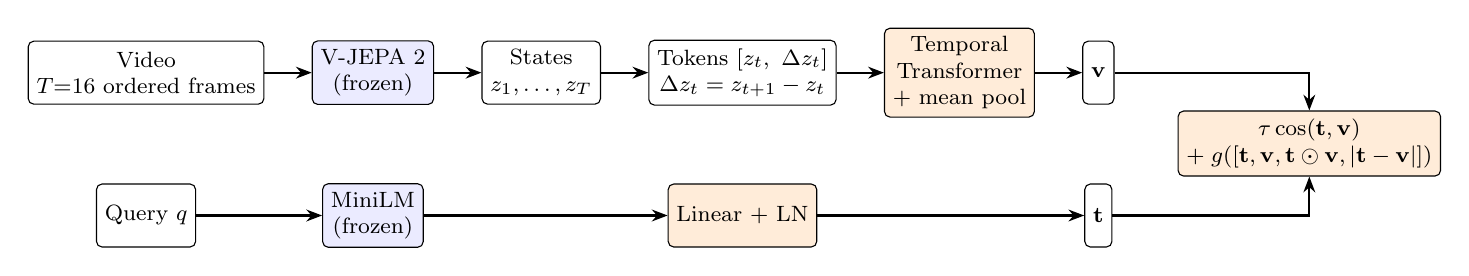
\begin{tikzpicture}[
  node distance=4mm and 6mm,
  box/.style={draw, rounded corners=2pt, align=center, minimum height=8mm,
              font=\footnotesize, inner sep=3pt},
  frozen/.style={box, fill=blue!8},
  learn/.style={box, fill=orange!15},
  arr/.style={-{Stealth[length=2mm]}, thick}]
  \node[box] (vid) {Video\\ $T{=}16$ ordered frames};
  \node[frozen, right=of vid] (enc) {V-JEPA 2\\ (frozen)};
  \node[box, right=of enc] (states) {States\\ $z_1,\dots,z_T$};
  \node[box, right=of states] (diff) {Tokens $[z_t,\ \Delta z_t]$\\ $\Delta z_t = z_{t+1}-z_t$};
  \node[learn, right=of diff] (tr) {Temporal\\ Transformer\\ + mean pool};
  \node[box, right=of tr] (v) {$\mathbf{v}$};
  \node[box, below=10mm of vid] (txt) {Query $q$};
  \node[frozen] (lm) at (enc |- txt) {MiniLM\\ (frozen)};
  \node[learn] (proj) at (diff |- txt) {Linear + LN};
  \node[box] (t) at (v |- txt) {$\mathbf{t}$};
  \node[learn, right=8mm of v, yshift=-9mm] (score)
       {$\tau\cos(\mathbf{t},\mathbf{v})$\\ $+\;g([\mathbf{t},\mathbf{v},\mathbf{t}\odot\mathbf{v},|\mathbf{t}-\mathbf{v}|])$};
  \draw[arr] (vid) -- (enc);
  \draw[arr] (enc) -- (states);
  \draw[arr] (states) -- (diff);
  \draw[arr] (diff) -- (tr);
  \draw[arr] (tr) -- (v);
  \draw[arr] (txt) -- (lm);
  \draw[arr] (lm) -- (proj);
  \draw[arr] (proj) -- (t);
  \draw[arr] (v) -| (score);
  \draw[arr] (t) -| (score);
\end{tikzpicture}
\caption{Overview of the proposed model. Blue blocks are frozen; orange blocks
are trained. Video states are computed once and cached, so training never
decodes video. \todo{Replace with a polished figure that shows example frames
and a pair of opposite actions (e.g., opening vs.\ closing) whose state sets
are similar but whose transition sequences differ.}}
\label{fig:pipeline}
\end{figure*}

\subsection{Frame Sampling and State Encoding}
We sample $T=16$ frames evenly over the clip and keep them in chronological
order. The clip is encoded by V-JEPA~2~\cite{assran2025vjepa2} (ViT-L,
checkpoint \texttt{vjepa2-vitl-fpc64-256}), which is kept frozen. V-JEPA~2
outputs patch tokens for each spatio-temporal tubelet of two frames. We average
the tokens over space within each tubelet, which gives $T/2$ temporal
features, and linearly interpolate them along time so that each sampled frame
receives one state $z_t\in\mathbb{R}^{D}$ with $D=1024$. States are computed
once per video and cached.

\subsection{Latent Transitions}
The change between consecutive states is
\begin{equation}
\label{eq:transition}
\Delta z_t = z_{t+1} - z_t, \qquad t = 1,\dots,T-1.
\end{equation}
Two properties make it a useful input. First, the transition sequence is
invariant to any component that is constant over the clip: if
$z_t = c + \tilde z_t$ for all $t$, then $\Delta z_t$ does not depend on $c$.
In the ideal case, this removes the background and the identity of the objects
and leaves their motion. Second, the order of $\Delta z_t$ is kept. Two
opposite actions such as ``picking something up'' and ``putting something
down'' visit similar states in reverse order; their transition sequences are
approximately reversed and negated, $\Delta z_t \mapsto -\Delta z_{T-t}$, and
are therefore easy to tell apart.

The first property is also a limitation for retrieval. SSv2 queries name
objects (``pulling mobile phone from left to right''), and a representation
built from transitions alone has discarded most of what identifies them. The
model therefore reads states and transitions together. Token $t$ is the
concatenation
\begin{equation}
\label{eq:token}
x_t = [\,z_t\,;\,\Delta z_t\,] \in \mathbb{R}^{2D}, \qquad t = 1,\dots,T-1,
\end{equation}
so the state supplies the scene content and the transition supplies the change
as an explicit signal that the encoder does not have to derive by comparing
positions. The last state is not a token of its own, but it is recoverable as
$z_{T-1}+\Delta z_{T-1}$. Feeding transitions alone is kept as an ablation
(Section~\ref{sec:ablation}).

The mean of the transitions telescopes,
\begin{equation}
\label{eq:telescope}
\frac{1}{T-1}\sum_{t=1}^{T-1}\Delta z_t = \frac{z_T - z_1}{T-1},
\end{equation}
so any order-insensitive pooling of $\Delta z_t$ only sees the net change
between the first and last frame. We use this identity to design ablations that
separate the contribution of the net change from that of the ordered sequence
(Section~\ref{sec:ablation}).

\subsection{Transition Encoder}
\label{sec:encoder}
In V-JEPA~2 feature space the states are about $6.5$ times larger in norm
than the transitions, so a single normalization over $x_t$ would let the state
dominate the token. The two halves are therefore layer-normalized separately
before a joint projection,
\begin{equation}
h_t^{(0)} = W\,[\,\mathrm{LN}_{z}(z_t)\,;\,\mathrm{LN}_{\Delta}(\Delta z_t)\,] + p_t,
\end{equation}
where $W\in\mathbb{R}^{d\times 2D}$, $d=256$, and $p_t$ is a learned position
embedding. A stack of $L=2$ pre-norm
Transformer encoder layers~\cite{vaswani2017attention} with 4 heads,
feed-forward width $4d$, and dropout $0.1$ lets each step attend to all others, so that the representation
of each step depends on what happened before and after it. The outputs
are mean-pooled over valid steps (padding is masked) and layer-normalized,
\begin{equation}
\mathbf{v} = \frac{\mathrm{LN}\!\left(\frac{1}{T-1}\sum_{t} h_t^{(L)}\right)}
                  {\left\|\mathrm{LN}\!\left(\frac{1}{T-1}\sum_{t} h_t^{(L)}\right)\right\|_2}.
\end{equation}
Because the inputs carry position embeddings and are mixed by self-attention
before pooling, $\mathbf{v}$ is sensitive to order even though the final
pooling is a mean. We refer to this as \emph{accumulating} the transitions.

\subsection{Text Encoder}
The query is encoded with the sentence encoder
all-MiniLM-L6-v2~\cite{wang2020minilm,reimers2019sbert}, which is kept frozen
and produces a 384-dimensional mean-pooled embedding $e_q$. A learned
projection maps it to the joint space,
$\mathbf{t} = \mathrm{LN}(U e_q)/\|\mathrm{LN}(U e_q)\|_2$ with
$U\in\mathbb{R}^{d\times 384}$. Each unique query string is encoded once.

\subsection{Query-Conditioned Scoring}
\label{sec:scoring}
The score combines a global similarity and a pairwise term:
\begin{equation}
\label{eq:score}
s(q,v) = \tau\,\mathbf{t}^{\top}\mathbf{v}
  + g\big([\,\mathbf{t};\,\mathbf{v};\,\mathbf{t}\odot\mathbf{v};\,|\mathbf{t}-\mathbf{v}|\,]\big),
\end{equation}
where $\tau = \min(e^{\theta}, 100)$ is a learned inverse temperature
initialized to $1/0.07$, and $g$ is a two-layer MLP
($4d\to 512\to 1$, GELU, dropout $0.1$). The cosine term alone yields a
standard dual encoder. The MLP looks at each query--video pair jointly, so the
same video embedding can be judged differently depending on which aspect of
the motion the query asks about. The element-wise product and absolute
difference are standard matching features for sentence-pair
models~\cite{reimers2019sbert}. The pairwise term costs $O(|\mathcal{Q}||\mathcal{V}|)$
MLP evaluations; for the gallery sizes in this paper (about $1.2\times10^4$ videos)
this is computed exactly in chunks. For larger galleries it can be applied as a
reranker to the top-$K$ results of the cosine term.
\todo{Report wall-clock scoring time per query and, if possible, a top-$K$
reranking variant.}

\subsection{Training Objective}
\label{sec:training}
SSv2 captions are template instantiations, so a mini-batch often contains
several videos with exactly the same caption. Let $S\in\mathbb{R}^{B\times B}$
be the score matrix of a batch with $S_{ij}=s(q_i,v_j)$, and let
$P_{ij}=1$ if $q_i$ and $q_j$ are the same string. We use a multi-positive
symmetric InfoNCE loss~\cite{oord2018cpc}:
\begin{equation}
\label{eq:loss}
\mathcal{L} = \frac{1}{2B}\sum_{i=1}^{B}\Big(
  \log\!\sum_{j} e^{S_{ij}} - \log\!\!\sum_{j:P_{ij}=1}\! e^{S_{ij}}
  + \log\!\sum_{j} e^{S_{ji}} - \log\!\!\sum_{j:P_{ji}=1}\! e^{S_{ji}}\Big).
\end{equation}
All pairs with the same caption are positives, so the model is never asked to
separate videos that the labels cannot distinguish. Only the transition
encoder, the text projection, the temperature, and the MLP $g$ are trained,
2.75M parameters in total.

% ===========================================================================
\section{Dataset and Evaluation Protocol}
\label{sec:data}
% ===========================================================================
\subsection{Something-Something V2 Retrieval Split}
SSv2~\cite{goyal2017ssv2} contains short clips of people performing one of
174 templated actions with everyday objects. Each clip has a caption in which
the template placeholders are replaced by object names, e.g., ``pulling mobile
phone from left to right.'' We use the caption as the text query and the clip
as its target. The official test labels are hidden, so we keep the official
training set and split the labeled official validation set 50/50 into a
development set and a held-out test set (entries sorted by video ID, then
permuted with seed 42). Table~\ref{tab:data} summarizes the result.

\begin{table}[!t]
\caption{Retrieval splits built from SSv2.}
\label{tab:data}
\centering
\begin{tabular}{lrrr}
\toprule
 & Train & Val & Test \\
\midrule
Videos / queries & 168{,}913 & 12{,}388 & 12{,}389 \\
Templates & 174 & 174 & 174 \\
Unique query strings & 109{,}968 & 10{,}179 & 10{,}087 \\
Queries with a duplicate string & 74{,}232 & 3{,}119 & 3{,}240 \\
Mean query length (words) & 6.6 & 6.4 & 6.4 \\
\bottomrule
\end{tabular}
\end{table}

\subsection{Full Retrieval}
Each test query is ranked against all 12{,}389 test videos. We report
Recall@$K$ ($K\in\{1,5,10\}$) and mean reciprocal rank (MRR), all in percent.
Each query has exactly one target video, so mean average precision equals MRR
and is not listed separately. Note that 3{,}240 test queries (26.2\%) share
their exact caption with at least one other test video. These videos are
indistinguishable from the text alone, but only the source video counts as
correct. A model that scores identical captions identically and breaks the tie
at random gets one expected hit per distinct caption, so its expected Recall@1
is at most $10{,}087/12{,}389 = 81.4\%$.
\todo{Optionally also report results where all videos with an identical
caption count as relevant.}

\subsection{Hard-Negative Retrieval}
\label{sec:hardneg}
To test whether a model understands \emph{what happens} rather than
\emph{what is shown}, each test query is also ranked against a small
candidate set of ten videos: its target plus nine negatives drawn from the
test split. Negatives never share the query's caption or action label, and
are chosen in order of priority:
\begin{enumerate}
\item \emph{Opposite action, same object}: videos whose action label is the
  opposite of the query's and whose primary (first annotated) object is the
  same.
\item \emph{Same objects, different action}: videos that share at least one
  annotated object with the query.
\item \emph{Other action}: any remaining video with a different action, used
  only to fill the set.
\end{enumerate}
The target is inserted at a random position. The selection uses a fixed seed
(42) and only the test split, so there is no overlap with training data.

\emph{Opposite actions.} Two labels count as opposites only if they appear in
a list of 21 label pairs that we wrote out and checked by hand, covering 38 of
the 174 labels. In each pair one action is the other reversed in time or
direction with the same kind of motion: opening/closing, covering/uncovering,
folding/unfolding, putting into/taking out of, picking up/putting on a
surface, moving up/down, pushing or pulling from left to right/right to left,
moving closer/away, and turning the camera left/right or up/down.
``Pretending'' labels are never paired, because they do not produce the real
state change. An explicit list replaced an earlier keyword rule that was too
permissive; for example, it paired every ``pulling'' label with every
``pushing'' label, including ones that move in the same direction.

Table~\ref{tab:hardneg} reports the composition. About 70\% of the distractors
share an object with the query, so appearance alone is of little help. Only
4.8\% are opposite actions, because few test videos show the opposite action
on the same primary object; 13.6\% of the queries have at least one.

\begin{table}[!t]
\caption{Composition of the hard-negative benchmark (test split).}
\label{tab:hardneg}
\centering
\begin{tabular}{lrr}
\toprule
 & Count & Share \\
\midrule
Queries & 12{,}389 & -- \\
Candidates per query & 10 & -- \\
Negatives in total & 111{,}501 & 100\% \\
\quad Opposite action, same object & 5{,}390 & 4.8\% \\
\quad Same objects, different action & 78{,}459 & 70.4\% \\
\quad Other action & 27{,}652 & 24.8\% \\
\midrule
Queries with $\geq$1 opposite-action negative & 1{,}688 & 13.6\% \\
Queries with $\geq$1 same-object negative & 10{,}511 & 84.8\% \\
Queries with only other-action negatives & 1{,}548 & 12.5\% \\
\bottomrule
\end{tabular}
\end{table}

\subsection{Action-Contrast Retrieval}
\label{sec:contrast}
Because opposite actions are a small share of the hard-negative set, its
aggregate score says little about direction. We therefore build a second
candidate set in which \emph{every} negative performs the opposite action and
there are no fillers. For each query, opposite-action videos with a different
caption are taken in three tiers: those with the same primary object first,
then those sharing any object, then the rest, so that appearance stays as
close to the target as the split allows. Queries whose action has no opposite
in the list are left out. This gives 3{,}793 queries (30.6\% of the test
split), each with its target and nine opposite-action negatives
(34{,}137 negatives in total). Of these negatives, 15.8\% share the query's
primary object, 6.0\% share another object, and 78.2\% share none.

\subsection{Candidate-Set Metrics}
With ten candidates, random ranking gives Recall@1 of 10.0\% and MRR of
29.3\% in both settings. We report Recall@1, Recall@5, and MRR. For the
hard-negative set we also report, per negative type, (i) the \emph{pairwise
accuracy}, the share of target--negative pairs in which the target scores
higher (ties count one half), and (ii) Recall@1 and MRR when the target is
ranked against only the negatives of that type. Pairwise accuracy has a chance
level of 50\% for every type and is comparable across types; the restricted
ranks are not, because the number of negatives per query differs.
\todo{Have a second annotator verify the 21 opposite pairs and a random sample
(e.g., 200) of opposite-action video pairs, and report agreement.}

% ===========================================================================
\section{Experiments}
\label{sec:experiments}
% ===========================================================================
\subsection{Implementation Details}
The main model, the trained baselines, and all ablations share one protocol.
Models are trained with AdamW~\cite{loshchilov2019adamw}
(learning rate $10^{-4}$, weight decay $0.01$) and batch size 128 for at most
50 epochs. Validation MRR on the full validation gallery is computed after
every epoch, training stops once it has not improved for 5 epochs, and the
checkpoint with the best validation MRR is evaluated once on the test split.
Every configuration is trained with three seeds (42, 43, 44); we report the
mean and the sample standard deviation over seeds. For the main model the best
epoch was 16, 20, and 19, and no run reached the epoch limit.

V-JEPA~2 and MiniLM are frozen, and their features are precomputed, so
training runs on cached features only. All 193{,}690 videos of the three
splits were decoded and encoded; none had to be dropped. One training run of
the main model, including test evaluation, takes under 30 minutes on a single
NVIDIA RTX~6000 Ada GPU. The trainable model has 2.75M parameters.
\todo{Number of GPUs and wall-clock time of feature extraction.}

\subsection{Baselines}
\begin{itemize}
\item \textbf{B1: CLIP frame averaging} (zero-shot). CLIP
  ViT-B/32~\cite{radford2021clip} encodes the 16 frames; their embeddings are
  averaged and compared with the CLIP text embedding of the query.
\item \textbf{B2: Pooled V-JEPA~2.} The 16 states are averaged into one
  vector, which is fed as a single token to the same encoder and trained as a
  dual encoder (no MLP term $g$) with the same recipe. This measures what the
  V-JEPA~2 features provide without temporal structure.
\item \textbf{B3: Transitions without query conditioning.} Our model with the
  MLP term $g$ removed from~\eqref{eq:score}, i.e., a dual encoder over the
  same $[z_t,\ \Delta z_t]$ tokens. B2 and B3 differ only in the video input;
  B3 and our model differ only in $g$.
\end{itemize}
\todo{Add at least one published text-video retrieval method trained on the
same split (e.g., CLIP4Clip~\cite{luo2022clip4clip} with sequential
Transformer pooling, and/or X-CLIP~\cite{ma2022xclip}). Reviewers at a
Transactions venue will expect this.}
\todo{Add a fine-tuned CLIP baseline so B1 is not only zero-shot.}

\subsection{Main Results}
Tables~\ref{tab:full} and~\ref{tab:hard} report full retrieval and the two
candidate-set settings. Our model reaches 9.9\% Recall@1 and 18.4\% MRR
against the full gallery of 12{,}389 videos, and the target is in the top ten
for 36.1\% of the queries. The spread over seeds is small (at most 0.2 points
in full retrieval). Full-gallery numbers are low in absolute terms, for two
reasons that are independent of temporal modeling: 26.2\% of the queries have
an identical caption elsewhere in the gallery
(Section~\ref{sec:data}), and telling apart thousands of everyday objects
relies on a frozen sentence encoder that was never aligned with video.

On the candidate sets the model is far above chance (10.0\% Recall@1,
29.3\% MRR): 77.1\% Recall@1 and 86.1\% MRR on hard negatives, and 73.9\%
Recall@1 and 83.3\% MRR when all nine distractors perform the opposite action.
Recall@5 is 98.2\% and 96.2\%, respectively, so the remaining errors are
confusions among the top few candidates.
\todo{Once the baselines have run, describe: (i) gain of B2 over B1
(self-supervised video features vs.\ image features); (ii) gain of B3 over B2
(effect of the ordered state--transition input); (iii) gain of ours over B3
(effect of query conditioning); (iv) whether the gaps widen on the
hard-negative and action-contrast sets, which is the central claim.}

\begin{table}[!t]
\caption{Full retrieval on the SSv2 test split (12{,}389 queries and videos),
in percent. Mean $\pm$ standard deviation over three seeds for trained models.
Best in bold.}
\label{tab:full}
\centering
\setlength{\tabcolsep}{3pt}
\begin{tabular}{lcccc}
\toprule
Model & R@1 & R@5 & R@10 & MRR \\
\midrule
B1: CLIP frame averaging & \tbd & \tbd & \tbd & \tbd \\
B2: V-JEPA~2, pooled & \tbd & \tbd & \tbd & \tbd \\
B3: Ours without $g$ & \tbd & \tbd & \tbd & \tbd \\
\todo{Published baseline} & \tbd & \tbd & \tbd & \tbd \\
\midrule
Ours & \ms{9.87}{0.19} & \ms{25.90}{0.12} & \ms{36.14}{0.18} & \ms{18.43}{0.11} \\
\bottomrule
\end{tabular}
\end{table}

\begin{table}[!t]
\caption{Candidate-set retrieval on the test split, in percent (10 candidates
per query; random: R@1 10.0, MRR 29.3). Hard negatives: 12{,}389 queries.
Action contrast: 3{,}793 queries, all negatives are opposite actions. Mean
$\pm$ standard deviation over three seeds for trained models. Best in bold.}
\label{tab:hard}
\centering
\setlength{\tabcolsep}{3pt}
\begin{tabular}{lcccc}
\toprule
 & \multicolumn{2}{c}{Hard negatives} & \multicolumn{2}{c}{Action contrast} \\
\cmidrule(lr){2-3}\cmidrule(lr){4-5}
Model & R@1 & MRR & R@1 & MRR \\
\midrule
B1: CLIP frame averaging & \tbd & \tbd & \tbd & \tbd \\
B2: V-JEPA~2, pooled & \tbd & \tbd & \tbd & \tbd \\
B3: Ours without $g$ & \tbd & \tbd & \tbd & \tbd \\
\todo{Published baseline} & \tbd & \tbd & \tbd & \tbd \\
\midrule
Ours & \ms{77.06}{0.14} & \ms{86.12}{0.14} & \ms{73.93}{0.78} & \ms{83.29}{0.49} \\
\bottomrule
\end{tabular}
\end{table}

\subsection{Ablation Study}
\label{sec:ablation}
Table~\ref{tab:ablation} varies the video input to the retrieval head, and in
one row the scorer; the training protocol and seeds follow the full model.
\begin{itemize}
\item \texttt{no\_transition}: the state sequence $z_{1..T}$ only.
\item \texttt{transition\_only}: the transition sequence $\Delta z_{1..T-1}$
  only.
\item \texttt{mean\_transition}: a single token, the mean of $\Delta z_t$.
\item \texttt{final\_minus\_initial}: a single token, $z_T - z_1$.
\item \texttt{no\_query\_conditioning}: the full $[z_t,\ \Delta z_t]$ tokens,
  MLP $g$ removed (identical to B3).
\end{itemize}
The first two rows split the full input into its halves. The gap between
\texttt{no\_transition} and the full model measures what the explicit
transition adds to a model that already sees the ordered states; the gap
between \texttt{transition\_only} and the full model measures what the scene
content adds. By~\eqref{eq:telescope}, \texttt{mean\_transition} and
\texttt{final\_minus\_initial} differ only by the factor $1/(T-1)$, which the
input LayerNorm removes. They should therefore score nearly the same, and
serve as a consistency check. Both keep only the net change and lose the order
of intermediate steps, so the gap between them and \texttt{transition\_only}
measures what the ordered sequence adds.
\todo{Interpret results once available.}

\begin{table}[!t]
\caption{Ablations on the video input and scoring (test split, MRR in
percent, mean $\pm$ standard deviation over three seeds).}
\label{tab:ablation}
\centering
\setlength{\tabcolsep}{2.5pt}
\begin{tabular}{lllccc}
\toprule
Variant & Video input & $g$ & Full & Hard & Contrast \\
\midrule
\texttt{no\_transition} & $z_{1..T}$ & \checkmark & \tbd & \tbd & \tbd \\
\texttt{transition\_only} & $\Delta z_{1..T-1}$ & \checkmark & \tbd & \tbd & \tbd \\
\texttt{mean\_transition} & $\overline{\Delta z}$ & \checkmark & \tbd & \tbd & \tbd \\
\texttt{final\_minus\_initial} & $z_T - z_1$ & \checkmark & \tbd & \tbd & \tbd \\
\texttt{no\_query\_cond.} & $[z_t,\Delta z_t]$ & -- & \tbd & \tbd & \tbd \\
\midrule
Full model & $[z_t,\Delta z_t]$ & \checkmark & \ms{18.43}{0.11} & \ms{86.12}{0.14} & \ms{83.29}{0.49} \\
\bottomrule
\end{tabular}
\end{table}

\todo{Additional ablations worth adding if compute allows: (a) number of
frames $T\in\{8,12,16\}$; (b) Transformer depth $L\in\{1,2,4\}$; (c) shuffled
or reversed token order at test time (a direct test of order
sensitivity); (d) one shared LayerNorm over $[z_t,\Delta z_t]$ instead of
separate ones; (e) a stronger or video-aligned text encoder instead of
MiniLM.}

% ===========================================================================
\section{Analysis}
\label{sec:analysis}
% ===========================================================================
\subsection{Which Distractors Are Hard?}
\label{sec:bytype}
Table~\ref{tab:bytype} breaks the hard-negative result of our model down by
negative type. The ordering is clear and stable across seeds. Fill-in
negatives with a different action and different objects are nearly solved
(98.6\% pairwise accuracy). Negatives that share an object with the query but
show a different action are beaten in 94.4\% of pairs. Opposite actions on the
same primary object are the hardest: the target wins only 83.5\% of these
pairs, about three times the error rate of same-object negatives.

The action-contrast set gives a complementary view. There the pairwise
accuracy against opposite-action negatives is $92.8\pm0.4$\%, clearly higher
than the 83.5\% above, although the action relation is the same. The
difference is the objects: in the hard-negative set every opposite-action
negative shares the query's primary object, whereas in the action-contrast
set only 15.8\% of the negatives do, and 78.2\% share no object with the query
at all, because the test split holds too few opposite-action videos of the
same object.
So part of what separates opposite actions in the action-contrast set is still
object identity, and the case in which only the direction of change differs
remains the main source of error.
\todo{Add the same breakdown for B1--B3. The claim of the paper is supported
if the opposite-action row improves most from B2 to ours.}

\begin{table}[!t]
\caption{Hard-negative results of our model by negative type (percent, mean
$\pm$ standard deviation over three seeds). Pair acc.: share of
target--negative pairs won by the target (chance 50). R@1 and MRR rank the
target against only the negatives of that type.}
\label{tab:bytype}
\centering
\setlength{\tabcolsep}{2.5pt}
\begin{tabular}{lrrccc}
\toprule
Negative type & Queries & Neg. & Pair acc. & R@1 & MRR \\
\midrule
Opposite action & 1{,}688 & 5{,}390 & \ms{83.49}{0.59} & \ms{74.51}{0.39} & \ms{84.53}{0.20} \\
Same objects & 10{,}511 & 78{,}459 & \ms{94.40}{0.18} & \ms{78.26}{0.14} & \ms{86.97}{0.16} \\
Other action & 4{,}085 & 27{,}652 & \ms{98.60}{0.02} & \ms{93.41}{0.07} & \ms{96.34}{0.02} \\
\bottomrule
\end{tabular}
\end{table}

\subsection{Error Categories}
For each failed query (target not ranked first), we compare the query with the
top-ranked wrong video using SSv2 templates, labels, and object names, and
assign one of seven categories: correct objects but wrong action, wrong
temporal direction, wrong action ordering, similar start and end but different
motion, text ambiguity (identical or near-identical captions), visual
ambiguity, and encoder failure. These rules sort failures for inspection; they
are heuristics, not ground truth.
Table~\ref{tab:errors} compares the error distribution of the baselines and
our model. \todo{Fill and interpret: the claim is supported if ``wrong temporal
direction'' and ``correct objects, wrong action'' errors drop most.}

\begin{table}[!t]
\caption{Error categories of failed queries in full retrieval (share of
failures, \%).}
\label{tab:errors}
\centering
\setlength{\tabcolsep}{3pt}
\begin{tabular}{lcccc}
\toprule
Category & B1 & B2 & B3 & Ours \\
\midrule
Correct objects, wrong action & \tbd & \tbd & \tbd & \tbd \\
Wrong temporal direction & \tbd & \tbd & \tbd & \tbd \\
Wrong action ordering & \tbd & \tbd & \tbd & \tbd \\
Similar start/end, different motion & \tbd & \tbd & \tbd & \tbd \\
Text ambiguity & \tbd & \tbd & \tbd & \tbd \\
Visual ambiguity & \tbd & \tbd & \tbd & \tbd \\
Encoder failure & \tbd & \tbd & \tbd & \tbd \\
\bottomrule
\end{tabular}
\end{table}

\subsection{Per-Template Analysis}
\todo{Plot per-template R@1 gain of ours over B2 for the 174 templates (sorted
bar chart), and highlight direction-sensitive templates (e.g., ``Pushing
something from left to right'' vs.\ ``from right to left'').}

\subsection{Qualitative Results}
\todo{Insert a figure (from \texttt{outputs/results/qualitative/}) showing
2--3 queries, the top-3 videos retrieved by B1 and by our model, with 4 frames
per video. Pick at least one opposite-action case.}

% ===========================================================================
\section{Limitations}
% ===========================================================================
\emph{Dataset scope.} SSv2 clips are short, recorded in controlled settings,
and captioned from 174 templates. Our results do not show that the method
transfers to open-domain search with free-form queries.
\todo{Strongly recommended for a journal: add at least one more benchmark,
e.g., a temporally sensitive one~\cite{bagad2023testoftime}, or
Charades~\cite{sigurdsson2016charades}/DiDeMo~\cite{hendricks2017didemo}, and
an appearance-driven one such as MSR-VTT~\cite{xu2016msrvtt} to show no loss.}

\emph{Frozen encoders.} V-JEPA~2 and MiniLM are frozen and states are
computed once at 16 frames. Fine-tuning the video encoder or sampling more
frames may change the conclusions. MiniLM is a general sentence encoder and is
not aligned with video; only the learned projection connects the modalities.

\emph{Appearance is still an input.} Because each token contains the state
$z_t$, the model can still rely on appearance; the transition is offered as an
additional signal, not enforced. The per-type results
(Section~\ref{sec:bytype}) show that opposite actions on the same object
remain the hardest case.

\emph{Linear transition operator.} The difference $z_{t+1}-z_t$ assumes that
change is approximately additive in V-JEPA~2's feature space and that adjacent
sampled frames show meaningful change. Very fast or very slow motion can break
both assumptions. Because states are interpolated from two-frame tubelets,
adjacent transitions within a tubelet are not independent.

\emph{Pairwise scoring cost.} The MLP term in~\eqref{eq:score} scales with the
product of the number of queries and videos, which limits exhaustive use on
very large galleries.

\emph{Candidate sets.} Opposite actions are defined by a list of 21 label
pairs that covers 38 of the 174 labels, so the action-contrast set evaluates
30.6\% of the test queries, and only 13.6\% of the queries have an
opposite-action negative in the hard-negative set.

% ===========================================================================
\section{Conclusion}
% ===========================================================================
We presented a text-to-video retrieval model that represents a video by an
ordered sequence of frozen V-JEPA~2 states paired with the transitions between
them. The state keeps the objects that queries name, and the separately
normalized transition makes the direction and order of change, which is what
distinguishes many actions in SSv2, an explicit input. With a
query-conditioned scorer and a multi-positive contrastive objective suited to
templated captions, the model reaches 9.9\% Recall@1 and 18.4\% MRR over a
gallery of 12{,}389 videos, with little variation over three seeds
\todo{and improves over the baselines by X}. On candidate sets it reaches
86.1\% MRR against hard negatives and 83.3\% MRR when every distractor
performs the opposite action, and a breakdown by distractor type shows that
opposite actions on the same object are still the hardest case. Future work
includes learned, non-linear transition operators, fine-tuning the video
encoder, a video-aligned text encoder, and evaluation on open-domain data with
free-form queries.

% ===========================================================================
\section*{Acknowledgments}
\todo{Acknowledge compute resources, funding, and contributors.}

% ===========================================================================
% References. Manual list in IEEE style, as in the official template.
% TODO: verify every entry (authors, venue, year, pages) before submission;
% consider switching to BibTeX with IEEEtran.bst.
% ===========================================================================
\begin{thebibliography}{99}

\bibitem{radford2021clip}
A.~Radford \textit{et~al.}, ``Learning transferable visual models from natural
language supervision,'' in \textit{Proc. Int. Conf. Mach. Learn. (ICML)},
2021, pp. 8748--8763.

\bibitem{luo2022clip4clip}
H.~Luo \textit{et~al.}, ``CLIP4Clip: An empirical study of CLIP for end to
end video clip retrieval and captioning,'' \textit{Neurocomputing}, vol.~508,
pp. 293--304, 2022.

\bibitem{ma2022xclip}
Y.~Ma, G.~Xu, X.~Sun, M.~Yan, J.~Zhang, and R.~Ji, ``X-CLIP: End-to-end
multi-grained contrastive learning for video-text retrieval,'' in
\textit{Proc. ACM Int. Conf. Multimedia}, 2022, pp. 638--647.

\bibitem{bain2021frozen}
M.~Bain, A.~Nagrani, G.~Varol, and A.~Zisserman, ``Frozen in time: A joint
video and image encoder for end-to-end retrieval,'' in \textit{Proc. IEEE/CVF
Int. Conf. Comput. Vis. (ICCV)}, 2021, pp. 1728--1738.

\bibitem{xu2016msrvtt}
J.~Xu, T.~Mei, T.~Yao, and Y.~Rui, ``MSR-VTT: A large video description
dataset for bridging video and language,'' in \textit{Proc. IEEE Conf. Comput.
Vis. Pattern Recognit. (CVPR)}, 2016, pp. 5288--5296.

\bibitem{buch2022atp}
S.~Buch, C.~Eyzaguirre, A.~Gaidon, J.~Wu, L.~Fei-Fei, and J.~C.~Niebles,
``Revisiting the `video' in video-language understanding,'' in \textit{Proc.
IEEE/CVF Conf. Comput. Vis. Pattern Recognit. (CVPR)}, 2022, pp. 2917--2927.

\bibitem{lei2023singleframe}
J.~Lei, T.~L.~Berg, and M.~Bansal, ``Revealing single frame bias for
video-and-language learning,'' in \textit{Proc. Annu. Meeting Assoc. Comput.
Linguistics (ACL)}, 2023.

\bibitem{bagad2023testoftime}
P.~Bagad, M.~Tapaswi, and C.~G.~M.~Snoek, ``Test of time: Instilling
video-language models with a sense of time,'' in \textit{Proc. IEEE/CVF Conf.
Comput. Vis. Pattern Recognit. (CVPR)}, 2023, pp. 2503--2516.

\bibitem{wang2023paxion}
Z.~Wang \textit{et~al.}, ``Paxion: Patching action knowledge in
video-language foundation models,'' in \textit{Adv. Neural Inf. Process.
Syst. (NeurIPS)}, 2023.

\bibitem{wang2016actions}
X.~Wang, A.~Farhadi, and A.~Gupta, ``Actions $\sim$ transformations,'' in
\textit{Proc. IEEE Conf. Comput. Vis. Pattern Recognit. (CVPR)}, 2016,
pp. 2658--2667.

\bibitem{assran2025vjepa2}
M.~Assran \textit{et~al.}, ``V-JEPA 2: Self-supervised video models enable
understanding, prediction and planning,'' arXiv:2506.09985, 2025.

\bibitem{goyal2017ssv2}
R.~Goyal \textit{et~al.}, ``The `something something' video database for
learning and evaluating visual common sense,'' in \textit{Proc. IEEE Int.
Conf. Comput. Vis. (ICCV)}, 2017, pp. 5842--5850.

\bibitem{miech2019howto100m}
A.~Miech, D.~Zhukov, J.-B.~Alayrac, M.~Tapaswi, I.~Laptev, and J.~Sivic,
``HowTo100M: Learning a text-video embedding by watching hundred million
narrated video clips,'' in \textit{Proc. IEEE/CVF Int. Conf. Comput. Vis.
(ICCV)}, 2019, pp. 2630--2640.

\bibitem{gabeur2020mmt}
V.~Gabeur, C.~Sun, K.~Alahari, and C.~Schmid, ``Multi-modal transformer for
video retrieval,'' in \textit{Proc. Eur. Conf. Comput. Vis. (ECCV)}, 2020,
pp. 214--229.

\bibitem{thrush2022winoground}
T.~Thrush \textit{et~al.}, ``Winoground: Probing vision and language models
for visio-linguistic compositionality,'' in \textit{Proc. IEEE/CVF Conf.
Comput. Vis. Pattern Recognit. (CVPR)}, 2022, pp. 5238--5248.

\bibitem{yuksekgonul2023aro}
M.~Yuksekgonul, F.~Bianchi, P.~Kalluri, D.~Jurafsky, and J.~Zou, ``When and
why vision-language models behave like bags-of-words, and what to do about
it?'' in \textit{Proc. Int. Conf. Learn. Represent. (ICLR)}, 2023.

\bibitem{simonyan2014twostream}
K.~Simonyan and A.~Zisserman, ``Two-stream convolutional networks for action
recognition in videos,'' in \textit{Adv. Neural Inf. Process. Syst. (NIPS)},
2014, pp. 568--576.

\bibitem{lin2019tsm}
J.~Lin, C.~Gan, and S.~Han, ``TSM: Temporal shift module for efficient video
understanding,'' in \textit{Proc. IEEE/CVF Int. Conf. Comput. Vis. (ICCV)},
2019, pp. 7083--7093.

\bibitem{zhou2018trn}
B.~Zhou, A.~Andonian, A.~Oliva, and A.~Torralba, ``Temporal relational
reasoning in videos,'' in \textit{Proc. Eur. Conf. Comput. Vis. (ECCV)}, 2018,
pp. 803--818.

\bibitem{feichtenhofer2019slowfast}
C.~Feichtenhofer, H.~Fan, J.~Malik, and K.~He, ``SlowFast networks for video
recognition,'' in \textit{Proc. IEEE/CVF Int. Conf. Comput. Vis. (ICCV)},
2019, pp. 6202--6211.

\bibitem{tong2022videomae}
Z.~Tong, Y.~Song, J.~Wang, and L.~Wang, ``VideoMAE: Masked autoencoders are
data-efficient learners for self-supervised video pre-training,'' in
\textit{Adv. Neural Inf. Process. Syst. (NeurIPS)}, 2022.

\bibitem{bardes2024vjepa}
A.~Bardes \textit{et~al.}, ``Revisiting feature prediction for learning
visual representations from video,'' \textit{Trans. Mach. Learn. Res.}, 2024.

\bibitem{mikolov2013linguistic}
T.~Mikolov, W.~Yih, and G.~Zweig, ``Linguistic regularities in continuous
space word representations,'' in \textit{Proc. NAACL-HLT}, 2013,
pp. 746--751.

\bibitem{vaswani2017attention}
A.~Vaswani \textit{et~al.}, ``Attention is all you need,'' in \textit{Adv.
Neural Inf. Process. Syst. (NIPS)}, 2017, pp. 5998--6008.

\bibitem{wang2020minilm}
W.~Wang, F.~Wei, L.~Dong, H.~Bao, N.~Yang, and M.~Zhou, ``MiniLM: Deep
self-attention distillation for task-agnostic compression of pre-trained
transformers,'' in \textit{Adv. Neural Inf. Process. Syst. (NeurIPS)}, 2020.

\bibitem{reimers2019sbert}
N.~Reimers and I.~Gurevych, ``Sentence-BERT: Sentence embeddings using
Siamese BERT-networks,'' in \textit{Proc. Conf. Empirical Methods Natural
Lang. Process. (EMNLP-IJCNLP)}, 2019, pp. 3982--3992.

\bibitem{oord2018cpc}
A.~van~den~Oord, Y.~Li, and O.~Vinyals, ``Representation learning with
contrastive predictive coding,'' arXiv:1807.03748, 2018.

\bibitem{loshchilov2019adamw}
I.~Loshchilov and F.~Hutter, ``Decoupled weight decay regularization,'' in
\textit{Proc. Int. Conf. Learn. Represent. (ICLR)}, 2019.

\bibitem{sigurdsson2016charades}
G.~A.~Sigurdsson, G.~Varol, X.~Wang, A.~Farhadi, I.~Laptev, and A.~Gupta,
``Hollywood in homes: Crowdsourcing data collection for activity
understanding,'' in \textit{Proc. Eur. Conf. Comput. Vis. (ECCV)}, 2016,
pp. 510--526.

\bibitem{hendricks2017didemo}
L.~A.~Hendricks, O.~Wang, E.~Shechtman, J.~Sivic, T.~Darrell, and B.~Russell,
``Localizing moments in video with natural language,'' in \textit{Proc. IEEE
Int. Conf. Comput. Vis. (ICCV)}, 2017, pp. 5803--5812.

\end{thebibliography}

% ===========================================================================
% Author biographies are required by most IEEE Transactions for the final
% version only. Uncomment and fill in when needed.
% ===========================================================================
% \begin{IEEEbiographynophoto}{Author One}
% Biography text here.
% \end{IEEEbiographynophoto}

\end{document}
